\chapter{Implementierung}
Das Verfahren wurde im Rahmen des Projektes in einen OpenGl C++ Programm umgesetzt.
Um die 2D Schatten zu implementieren müssen zwingend Framebuffer benutzt werden.
Den ohne können die entsprechenden Texturen nicht erstellt werden die zu Berechnung der Schatten benötigt werden. 
\begin{figure}
	\centering
	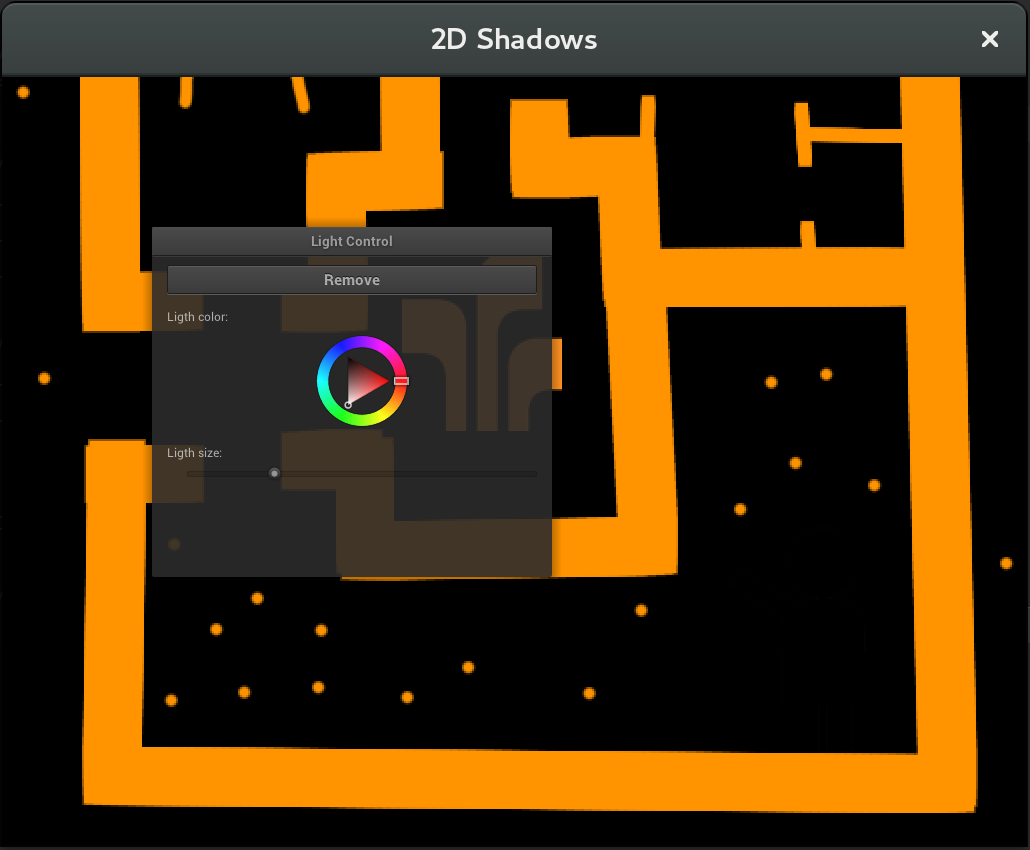
\includegraphics[scale=0.25]{images/Bildschirmfoto_1.png}
	\caption{Programm beim nach dem Start.}
	\label{p_1}
\end{figure}

Die Schritte die hier beschrieben werden müssen für jedes Licht durchgeführt werden.

\section{Oclussionmap}

Für die Oclussionmap wird eine Textur angelegt die der Größe des Lichtes entspricht.
\begin{lstlisting}
	// The texture we're going to render to
	GLuint oclusion_texture;
	glGenTextures(1, &oclusion_texture);
	
	// "Bind" the newly created texture : 
	// all future texture functions will modify this texture
	glBindTexture(GL_TEXTURE_2D, oclusion_texture);
	
	// Give an empty image to OpenGL ( the last "0" )
	glTexImage2D(GL_TEXTURE_2D, 0,GL_RGBA8,
				 ligthsize, ligthsize, 0,
				 GL_RGBA, GL_UNSIGNED_BYTE, 0);
\end{lstlisting}

Diese wird nun an ein FBO gebunden.
\begin{lstlisting}
// Set "oclusion_texture" as our colour attachement #0
glFramebufferTexture(GL_FRAMEBUFFER, GL_COLOR_ATTACHMENT0, 
					 oclusion_texture, 0);
\end{lstlisting}

Jetzt müssen die Occluder nur noch entsprechen transformiert gerendert werden.
\begin{lstlisting}
auto mvp = glm::mat4{1};
auto ligthsize_half = (ligthsize/2.f);
mvp = glm::ortho(0.f, float(ligthsize), 0.f, float(ligthsize));
mvp *= glm::translate(glm::mat4{1},
			glm::vec3(-pos.x+ligthsize_half,-pos.y+ligthsize_half,0));
render_ocluders(mvp);
\end{lstlisting}

Dabei wird kein Spezieller Shader benutzt es ist nur wichtig das die Alphakanal Informationen vorhanden sind.

\section{Shadowmap}

